\documentclass{jlreq}

\RequirePackage{calc}
\RequirePackage{tikz}
\RequirePackage{KKsymbols}
\usetikzlibrary{shapes}
\usetikzlibrary{calc}

\usepackage{KKran}

\makeatletter
% %=== シルエット生成用パッチ ===
% \newcommand{\BlockFillMode}{%
%   % 1. カウンターが進まないようにローカル化(または無効化)したいが、
%   %    位置計算に使うためそのまま走らせ、表示だけ消す戦略をとります。
%   %    ただし、文字出力(\kakkoなど)は空にします。
%   \def\kakko##1{}%
%   \def\KaitouInput##1{}%
  
%   % 2. 各ボックス描画コマンドを「矩形塗りつぶし(\fill)」に再定義
%   %    ※位置計算(pgfmath...)はstyからコピーして維持します
  
%   % --- Daimon@Box@A@N のパッチ ---
%   \RenewDocumentCommand{\Daimon@Box@A@N}{ O{.7pt} m m }{%
%     \fill (\mondai@position@tmp\width@KKran,-\mondai@position@y@tmp\width@KKran) 
%           rectangle ++(##2\width@KKran, -##3\width@KKran);%
%     \pgfmathparse{\mondai@position@tmp + \modai@bangou@wd}%
%     \edef\mondai@position@tmp{\pgfmathresult}%
%   }%
  
%   % --- Shoumon@Box@A@N のパッチ ---
%   \RenewDocumentCommand{\Shoumon@Box@A@N}{ O{.7pt} O{.35pt} O{.5} m }{%
%     \fill (\mondai@position@tmp\width@KKran,-\mondai@position@y@tmp\width@KKran) 
%           rectangle ++(##3\width@KKran, -##4\width@KKran);%
%     \pgfmathparse{\mondai@position@tmp + ##3}%
%     \edef\mondai@position@tmp{\pgfmathresult}%
%   }%
  
%   % --- Shoumon@Box@A のパッチ ---
%   \RenewDocumentCommand{\Shoumon@Box@A}{ O{.7pt} O{.35pt} m m O{} }{%
%     \fill (\mondai@position@tmp\width@KKran,-\mondai@position@y@tmp\width@KKran) 
%           rectangle ++(##3\width@KKran, -##4\width@KKran);%
%     \pgfmathparse{\mondai@position@tmp + ##3}%
%     \edef\mondai@position@tmp{\pgfmathresult}%
%   }%

%   % --- Shoumon@Grid@A / NonGrid などの複雑なものは
%   %     「外枠の矩形」だけ塗りつぶす簡易版に置き換えます
%   %     (厳密なGrid計算が必要な場合はstyのロジックをコピーする必要がありますが、
%   %      ここでは「幅(#3)×高さ(1単位)」と仮定しています。必要に応じて調整してください)
%   \RenewDocumentCommand{\Shoumon@NonGrid@A}{ O{.7pt} O{.35pt} m}{%
%      \fill (\mondai@position@tmp\width@KKran,-\mondai@position@y@tmp\width@KKran) 
%            rectangle ++(##3\width@KKran, -1\unit@KKran);% ※高さが可変の場合は要調整
%      \pgfmathparse{\mondai@position@tmp + ##3}%
%      \edef\mondai@position@tmp{\pgfmathresult}%
%   }%
%   \RenewDocumentCommand{\Shoumon@Grid@A}{ O{.7pt} O{.35pt} m O{##3}}{%
%      \fill (\mondai@position@tmp\width@KKran,-\mondai@position@y@tmp\width@KKran) 
%            rectangle ++(##3\width@KKran, -1\unit@KKran);% ※高さ固定と仮定
%      \pgfmathparse{\mondai@position@tmp + ##3}%
%      \edef\mondai@position@tmp{\pgfmathresult}%
%   }%
% }
\makeatother

\makeatletter

\begin{document}

\KKran[3pt]{%
  \Daimon@Box@A@N{.5}{7}%
  \Shoumon@Box@A@N{2}\Shoumon@Box@A{5}{2}\Shoumon@Box@A@N{2}\Shoumon@Box@B{3}{2}\Shoumon@Box@A{3}{2}\GoDown{2}
  \Shoumon@Box@A@N{2}\Shoumon@Box@A{3}{2}\Shoumon@Box@A@N{2}\Shoumon@Box@A{5}{2}\Shoumon@Box@A@N{2}\Shoumon@Box@A{3}{2}\GoDown{2}\Shoumon@Box@A@N{3}\Shoumon@NonGrid@A{45}[37]
}

\KKran{%
  \Daimon@Box@A@N{.5}{5}%
  \Shoumon@Box@A@N{2}\Shoumon@Box@A{3}{2}\Shoumon@Box@A@N{2}\Shoumon@Box@A{5}{2}\Shoumon@Box@A@N{2}\Shoumon@Box@A{3}{2}\GoDown{2}
  \Shoumon@Box@A@N{2}\Shoumon@Box@A{3}{2}[south east=$\mathrm{mm}$]\Shoumon@Box@A@N{2}\Shoumon@Box@A{5}{2}\Shoumon@Box@A@N{2}\Shoumon@Box@A{3}{2}\GoDown{2}
  \Shoumon@Box@A@N{1}{1}\Shoumon@NonGrid@A{5}\Shoumon@Box@A@N{2}\Shoumon@Box@A{3}{2}\Shoumon@Box@A@N{1}{1}\Shoumon@Grid@A{5}[3]
}


\begin{tikzpicture}
  \Daimon@Box@A@N{.5}{5}%
  \Shoumon@Box@A@N{2}\Shoumon@Box@A{3}{2}\Shoumon@Box@A@N{2}\Shoumon@Box@A{5}{2}\Shoumon@Box@A@N{2}\Shoumon@Box@A{3}{2}\GoDown{2}
  \Shoumon@Box@A@N{2}\Shoumon@Box@A{3}{2}[south east=$\mathrm{mm}$]\Shoumon@Box@A@N{2}\Shoumon@Box@A{5}{2}\Shoumon@Box@A@N{2}\Shoumon@Box@A{3}{2}\GoDown{2}
  \Shoumon@Box@A@N{1}{1}\Shoumon@NonGrid@A{5}\Shoumon@Box@A@N{2}\Shoumon@Box@A{3}{2}\Shoumon@Box@A@N{1}{1}\Shoumon@Grid@A{5}[3]
\end{tikzpicture}

\begin{tikzpicture}
  \Daimon@Box@A@N{.5}{7}%
  \Shoumon@Box@A@N{2}\Shoumon@Box@A{5}{2}\Shoumon@Box@A@N{2}\Shoumon@Box@B{3}{2}\Shoumon@Box@A{3}{2}\GoDown{2}
  \Shoumon@Box@A@N{2}\Shoumon@Box@A{3}{2}\Shoumon@Box@A@N{2}\Shoumon@Box@A{5}{2}\Shoumon@Box@A@N{2}\Shoumon@Box@A{3}{2}\GoDown{2}\Shoumon@Box@A@N{3}\Shoumon@NonGrid@A{47}
\end{tikzpicture}
\end{document}


% タスク
% 縦書きの時は問題番号のところを90度回転。
% 上下右のどこを点線にするかをkeyvalで。
% 上下左右どこを太線にするのかをkeyvalで設定できるように。
% 各コマンドの引数はkeyvalに。